\citet{mcdonald2007structured} uvode jednostavan model za označavanje sentimenta
kroz više razina. Koristeći njihov model moguće je združeno za jedan dokument
označiti njegov sentiment, ali i sentiment paragrafa i rečenica u dokumentu. Ako
bi se sentiment označavao tako da se prvo označi sentiment dokumenta, pa se ta
informacija propagira na niže razine, onda doći će do nakupljanja pogrešaka jer
učenje nije provedeno združeno. Na slici \ref{fig:sentimentmodels} prikazana su
dva modela, slika \ref{fig:sentimentmodels:docsent} pokazuje vjerojatnosni
grafički model u slučaju označavanja sentimenta dokumenta i rečenica, a slika
\ref{fig:sentimentmodels:docparsent} dodatno označavanje i paragrafa. Ako
pretpostavimo da je broj mogućih oznaka sentimenta jednak za sve razine, onda je
vremenska složenost koraka učenja i predviđanja za model na prvoj slici $O(M^3
T)$, a $O(M^4 P T)$ za model na drugoj -- gdje je $M$ broj mogućih oznaka
sentimenta, $P$ broj paragrafa u dokumentu i $T$ broj rečenica u dokumentu. Ako
bi htjeli dodati broj prijašnjih odluka koje utječu na trenutnu, onda bi
eksponent na $M$ rastao. Ako bi se broj mogućih oznaka povećao, onda bi se
učenje i zaključivanje dodatno usporilo. Već sada se može zaključiti da učenje i
zaključivanje rađeno u okviru vjerojatnosnih grafičkih modela neće biti dovoljno
brzo.

Korisno je razmotriti isti problem u okviru učenja pretraživanja. U dodatku
\ref{appendix:sentiment} prisutne su dvije moguće implementacije u okviru učenja
pretraživanja za model označavanja sentimenta i rečenica. Moguće je donositi
odluke na dva načina:
\begin{inlinelist}
  \item prvo odrediti sentiment na dokumentu pa onda propagirati tu informaciju
  pri donošenju odluka na rečenicama,
  \item prvo odrediti sentiment na svim rečenicama pa onda propagirati cijeli
  određeni sentiment na odluku za dokument.
\end{inlinelist}
Algoritam \ref{alg:sentiment:docsent} ilustrira prvi pristup, a ponašanje
funkcija identično je kao i u algoritmima u potpoglavlju \ref{ch:postaggingapp}.
Očigledno je postupak određivanja sentimenta samo na rečenicama jednak običnom
označavanju niza stoga se implementacija na ovom zadatku ne razlikuje previše od
običnog označivača niza. Drugi pristup ima manu što se ovisno o broju rečenica u
dokumentu raste broj značajki za odluku na razini dokumenta (svaka odluka na
rečenici postaje značajka u odluci za dokument). Prvi pristup koristi se u
\citet{mcdonald2007structured}. Lakše je odrediti sentiment za cijeli dokument
nego prvo za rečenice. Vremenska složenost ovog pristupa je iznenađujuće dobra.
Zaključivanje ima vremensku složenost $O(M (P + T))$ za model na slici
\ref{fig:sentimentmodels:docparsent}. Ogromna razlika u usporedbi s
vjerojatnosnim grafičkim modelom.

\begin{algorithm}
\caption{Združena analiza sentimenta dokumenta i rečenica.}
\label{alg:sentiment:docsent}
\begin{algorithmic}[1]
\Function{\textsc{Run}}{dokument}
\State $\textit{izlaz} \gets \text{[]}$
\State \textit{dlabel} $\gets$ \Call{Predict}{dokument, dokument.točna\_oznaka}
\For{$n \gets 1$ \textbf{do} \Call{Len}{dokument}}
  \State \textit{ref} $\gets$ \text{dokument[n].točna\_oznaka}
  \State \textit{izlaz[n]} $\gets$ \Call{Predict}{dokument[n], ref, izlaz[:n-1], dlabel}
\EndFor
\State \Call{Gubitak}{\# izlaz[n] $\neq$ dokument[n].točna\_oznaka}
\State \textbf{return} izlaz
\EndFunction
\end{algorithmic}
\end{algorithm}

Ovaj pristup lako je primijeniti i na hijerarhijsko označavanje kategorije
dokumenata. Prednost pristupa je taj što metoda učenja pretraživanja ima
garancije da akumulirana pogreška ne ovisi o duljini niza odluka, a uvjetovanje
na prošle odluke se ostvaruje samo dodavanjem dodatnih značajki. Vremenska
složenost je dodatna prednost.

\begin{figure}
\tikzstyle{undirect}=[shape=rectangle,draw=black,fill=black]

\begin{subfigure}[b]{1\textwidth}
\begin{center}
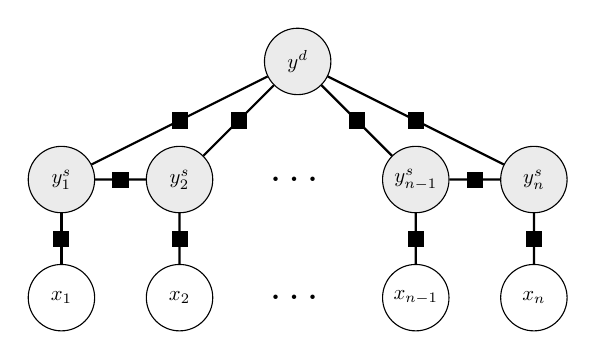
\begin{tikzpicture}[scale=0.75,every node/.style={transform shape}]
\tikzstyle{state}=[shape=circle,draw=black,fill=black!8,minimum size=32pt]
\tikzstyle{observation}=[shape=circle,draw=black,fill=white!20,minimum size=32pt]
% states
\node[state] (yd) at (5,5) {$y^{\text{d}}$};

\node[state] (ys1) at (1,3) {$y^{\text{s}}_1$};
\node[state] (ys2) at (3,3) {$y^{\text{s}}_2$};
\node[state] (ys3) at (7,3) {$y^{\text{s}}_{n-1}$};
\node[state] (ys4) at (9,3) {$y^{\text{s}}_{n}$};

% observations
\node[observation] (x1) at (1,1) {$x_{1}$}
    edge [thick] node[undirect] {} (ys1);
\node[observation] (x2) at (3,1) {$x_{2}$}
    edge [thick] node[undirect] {} (ys2);
\node[observation] (x3) at (7,1) {$x_{n-1}$}
    edge [thick] node[undirect] {} (ys3);
\node[observation] (x4) at (9,1) {$x_{n}$}
    edge [thick] node[undirect] {} (ys4);

\draw[thick] (ys1) edge node[undirect] {} (ys2);
\draw[thick] (ys3) edge node[undirect] {} (ys4);

\draw[thick] (yd) edge node[undirect] {} (ys1);
\draw[thick] (yd) edge node[undirect] {} (ys2);
\draw[thick] (yd) edge node[undirect] {} (ys3);
\draw[thick] (yd) edge node[undirect] {} (ys4);
\draw (ys2) edge[draw=none] node[scale=2] {\ldots} (ys3);
\draw (x2) edge[draw=none] node[scale=2] {\ldots} (x3);

\end{tikzpicture}
\caption{Model za određivanje sentimenta rečenica i dokumenta.}
\label{fig:sentimentmodels:docsent}
\end{center}
\end{subfigure}

\begin{subfigure}[b]{1\textwidth}
\centering
\begin{tikzpicture}[scale=0.75,every node/.style={transform shape}]
\tikzstyle{state}=[shape=circle,draw=black,fill=black!8,minimum size=32pt]
\tikzstyle{observation}=[shape=circle,draw=black,fill=white!20,minimum size=32pt]
% document
\node[state] (yd) at (10,7) {$y^{\text{d}}$};

% paragraph 1
\node[state] (yp1) at (5,5) {$y^{\text{p}}_{1}$};

\node[state] (ys1) at (1,3) {$y^{\text{s,1}}_1$};
\node[state] (ys2) at (3,3) {$y^{\text{s,1}}_2$};
\node[state] (ys3) at (7,3) {$y^{\text{s,1}}_{m-1}$};
\node[state] (ys4) at (9,3) {$y^{\text{s,1}}_{m}$};

% observations
\node[observation] (p1x1) at (1,1) {$x^{1}_{1}$}
    edge [thick] node[undirect] {} (ys1);
\node[observation] (p1x2) at (3,1) {$x^{1}_{2}$}
    edge [thick] node[undirect] {} (ys2);
\node[observation] (p1x3) at (7,1) {$x^{1}_{n-1}$}
    edge [thick] node[undirect] {} (ys3);
\node[observation] (p1x4) at (9,1) {$x^{1}_{n}$}
    edge [thick] node[undirect] {} (ys4);

\draw[thick] (ys1) edge node[undirect] {} (ys2);
\draw[thick] (ys3) edge node[undirect] {} (ys4);

\draw[thick] (yp1) edge node[undirect] {} (ys1);
\draw[thick] (yp1) edge node[undirect] {} (ys2);
\draw[thick] (yp1) edge node[undirect] {} (ys3);
\draw[thick] (yp1) edge node[undirect] {} (ys4);
\draw (ys2) edge[draw=none] node[scale=2] {\ldots} (ys3);
\draw (x2) edge[draw=none] node[scale=2] {\ldots} (x3);

%% paragraph 2
\node[state] (yp2) at (15,5) {$y^{\text{p}}_{k}$};

\node[state] (p2ys1) at (11,3) {$y^{\text{s,k}}_1$};
\node[state] (p2ys2) at (13,3) {$y^{\text{s,k}}_2$};
\node[state] (p2ys3) at (17,3) {$y^{\text{s,k}}_{l-1}$};
\node[state] (p2ys4) at (19,3) {$y^{\text{s,k}}_{l}$};

% observations
\node[observation] (p2x1) at (11,1) {$x^{k}_{1}$}
    edge [thick] node[undirect] {} (p2ys1);
\node[observation] (p2x2) at (13,1) {$x^{k}_{2}$}
    edge [thick] node[undirect] {} (p2ys2);
\node[observation] (p2x3) at (17,1) {$x^{k}_{l-1}$}
    edge [thick] node[undirect] {} (p2ys3);
\node[observation] (p2x4) at (19,1) {$x^{k}_{l}$}
    edge [thick] node[undirect] {} (p2ys4);

\draw[thick] (p2ys1) edge node[undirect] {} (p2ys2);
\draw[thick] (p2ys3) edge node[undirect] {} (p2ys4);

\draw[thick] (yp2) edge node[undirect] {} (p2ys1);
\draw[thick] (yp2) edge node[undirect] {} (p2ys2);
\draw[thick] (yp2) edge node[undirect] {} (p2ys3);
\draw[thick] (yp2) edge node[undirect] {} (p2ys4);
\draw (p2ys2) edge[draw=none] node[scale=2] {\ldots} (p2ys3);
\draw (p2x2) edge[draw=none] node[scale=2] {\ldots} (p2x3);

% from document to paragraph
\draw[thick] (yd) edge node[undirect] {} (yp1);
\draw[thick] (yd) edge node[undirect] {} (yp2);
\draw (yp1) edge[draw=none] node[scale=2] {\ldots\quad\ldots\quad\ldots} (yp2);

\end{tikzpicture}
\caption{Model za određivanje sentimenta rečenica, paragrafa i dokumenta.}
\label{fig:sentimentmodels:docparsent}
\end{subfigure}

\caption[Prikaz hijerarhijskih sentiment modela.]{Prikaz hijerarhijskih
sentiment modela. Sivi čvorovi predstavljaju varijable koje model može
generirati, a bijeli koje model može samo opaziti. Prikazana su dva modela gdje
su ulazi modelirani značajkama, a izlazi su kategoričke varijable sentimenta
(pozitivno, negativno i neutralno). Varijable dokumenta $y^{\text{d}}$,
paragrafa $y^{\text{p}}$ i rečenice $y^{\text{s}}$ predstavljaju sentiment, a
$x_i$ ulaznu rečenicu.}
\label{fig:sentimentmodels}
\end{figure}
